\documentclass{standalone}
\usepackage{tikz}
\usepackage{ctex,siunitx,ninecolors}
\setCJKmainfont{Noto Serif CJK SC}
\setCJKsansfont{Noto Sans CJK SC}
\usepackage{tkz-euclide}
\usepackage{amsmath}
\usetikzlibrary{patterns, calc}
\usetikzlibrary {decorations.pathmorphing, decorations.pathreplacing, decorations.shapes,}
\begin{document}
\small
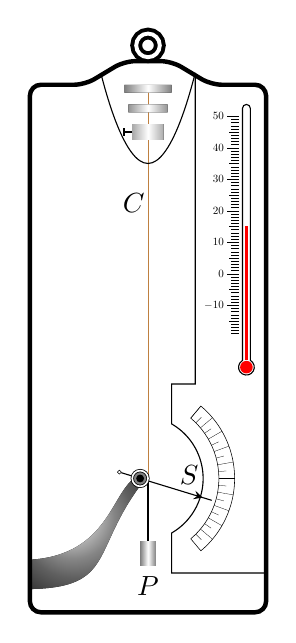
\begin{tikzpicture}[>=latex,scale=1.0,inner sep =1pt]
  % \useasboundingbox(-1.4,-1.4)rectangle(1.4,1.4);
  \draw[brown,very thin](0,5)--(0,0);
  \draw(0,-0.8)--(0,0);
  \fill[left color=gray,right color=gray,middle color=white](-0.1,-0.8)rectangle(0.1,-1.1);
  \node at (0,-1.2)[below]{$P$};
  \node at (0,3.5)[left]{$C$};
  \fill[ball color=lightgray](-1.500,-1.405)..controls(-0.409,-1.384)and(-0.729,-0.911)..
  (-0.065,-0.046)..controls(-0.047, 0.008)and(-0.079, 0.046)..
  (-0.134, 0.028)..controls(-0.467,-0.143)and(-0.480,-0.973)..(-1.500,-1.032);
  \begin{scope}[xshift=-1mm]
  \foreach \x in {50,40,...,-40}
  {
    \draw[ultra thin] (\x:1.0)--(\x:1.2);
    \draw[ultra thin] (\x-5:1.0)--(\x-5:1.1);
  }
  \draw[very thin](-50:1.0)--(-50:1.2)arc(-50:50:1.2)--(50:1.0)arc(50:-50:1.0);
  \draw(0.7,5.15)--(0.7,1.2)--(0.4,1.2)--(60:0.8)arc(60:-60:0.8)--(0.4,-1.2)--(1.6,-1.2);
  \draw(-0.5,5.15) parabola bend (0.1,4.0) (0.7,5.15);
  
  \draw[postaction={decorate},decoration={markings,mark=at position 0.9 with {\arrow{stealth}}}](163:0.25)--(-17:0.95)node[pos=0.75,above=2pt]{$S$};
  \draw[very thin](163:0.275)circle(0.025);
  \draw[double,line width=0.1mm,fill=gray](0,0)circle(0.1);
  \fill(0,0)circle(0.05);
  \end{scope}
  \fill[left color=gray,right color=gray,middle color=white](-0.2,4.5)rectangle(0.2,4.3)(-0.25,4.75)rectangle(0.25,4.65)(-0.3,5.0)rectangle(0.3,4.9);
  \draw[thick](-0.2,4.4)--(-0.3,4.4)(-0.3,4.45)--(-0.3,4.35);
  \foreach \y[count=\i] in {50,40,30,20,10,0,-10}
  {
    \draw[ultra thin](1.15,5.0-0.4*\i)--++(-0.15,0)node[left]{\scalebox{0.4}{$\y$}}; 
    \draw[ultra thin](1.15,5.0-0.4*\i-0.2)--++(-0.12,0);
    \foreach \z in {1,2,3,4,6,7,8,9}
    {\draw[ultra thin](1.15,5.0-0.4*\i-0.04*\z)--++(-0.10,0);}
  }
  \draw(1.2,4.7)arc(180:0:0.05)--(1.3,1.5)arc(420:120:0.1)--cycle;
  \fill[red](1.25,1.4134)circle(0.08);
  \draw[red,thick](1.25,1.5)--(1.25,3.2);
  \draw[ultra thick,rounded corners](-1.5,-1.7)--(1.5,-1.7)--(1.5,5)--(0.8,5)--(0.3,5.3)--(-0.3,5.3)--(-0.8,5)--(-1.5,5)--cycle;
  \draw[double,double distance=0.5mm, line width=0.5mm](0,5.5)circle(0.15);
\end{tikzpicture}
\end{document}